\section{Organization of the input and output data}
\label{sec:data_organization}

\gb
Working with LANS, and with nanoSIMS data in general, can be a book-keeping challenge. To start with, you will have many raw data files (\ttt{im} or \ttt{im.zip} files) acquired at different dates and from different types of samples (e.g., different treatments). Additionally, processing of those raw data files with LANS will create many output files, including data in a~standard text format (ASCII), PDF images, matlab output, PDF output, and zipped backed-up folders. It is therefore a good idea to develop and maintain a certain structure of those folders and output files, to \emph{keep everything organized}. 
\gbe

In this document, we assume that the raw and processed nanoSIMS data are organized hierarchically as shown in Table~\ref{tab1:file_structure}. We have used this data organization at Utrecht University for many years, and it works pretty well. We therefore highly encourage users to adopt it as well. Its benefits will become more apparent later on, when we get to the point of explaining how to efficiently process and analyze \emph{multiple} nanoSIMS datasets from a particular project.

\begin{table}[!t]
\centering
\caption{\label{tab1:file_structure} Hierarchical organization of the raw and processed nanoSIMS data implemented in Look@NanoSIMS. An example of such data organization along with a more detailed explanation is shown in Figures~\ref{fig2:data_organizationAB} and~\ref{fig2:data_organizationCD}.}
\begin{tabular}{l@{ $\rightarrow$ }c@{ $\rightarrow$ }l@{ $\rightarrow$ }l@{ $\rightarrow$ }l}
\hline
root & project & measurment day 1 & raw dataset 1.1 & \color{red}{dataset folder} 1.1\\
\multicolumn{2}{c}{} & & raw dataset 1.2  & dataset folder 1.2\\
\multicolumn{2}{c}{} & & $\cdots$ & $\cdots$ \\
\multicolumn{1}{c}{} & & measurement day 2 & raw dataset 2.1  & dataset folder 2.1\\
\multicolumn{2}{c}{} & & raw dataset 2.2  & dataset folder 2.2\\
\multicolumn{2}{c}{} & & $\cdots$ & $\cdots$\\
\multicolumn{1}{c}{} & & $\cdots$ & $\cdots$ & $\cdots$\\
\hline
\multicolumn{2}{r}{\color{red}{dataset folder} $i$ $\rightarrow$} & \color{orange}{dat} & \multicolumn{2}{l}{\color{orange}{numbers in a text format}} \\
\multicolumn{2}{r}{$\rightarrow$} & \textcolor{darkgold}{pdf} & \multicolumn{2}{l}{\textcolor{darkgold}{images \&\ graphs in a pdf format}} \\
\multicolumn{2}{r}{$\rightarrow$} & \multicolumn{3}{l}{\hspace{-2mm}processing definition files (\textcolor{purple}{alignment, ROIs, preferences})} \\
\multicolumn{2}{r}{$\rightarrow$} & \multicolumn{3}{l}{\hspace{-2mm}\textcolor{purple}{OutputG.pdf (output summary)}}\\
\hline
\end{tabular}
\end{table}

At the highest level of the data organization is a root folder that contains \emph{all} nanoSIMS data. This folder contains `project folders' with nanoSIMS data belonging to \emph{specific projects}. Each `project folder' contains `day folders' with data acquired on \emph{different measurement days}. Each `day folder' contains the actual \emph{raw datasets} (\ttt{im} or \ttt{im.zip} files). When a particular raw dataset is processed and analyzed, the corresponding data is stored in a `dataset folder' with the \emph{same name} as the dataset. Each `dataset folder' contains sub-folders with the \emph{results} of the analysis, including numerical values such as ROI-specific ion counts or ion count ratios, stored in sub-folder \ttt{dat}, and graphical output such as images or scatter plots stored in sub-folder \ttt{pdf}. The `dataset folder' also contains information defining the processing steps, such as alignment of planes, definition and classification of regions of interest (ROIs), and preferences. This information is useful if you want to go back to the analysis of the same dataset after you have analyzed a different one, e.g., to perform quality checks or more in-depth analyses. Finally, the `dataset folder' also contains a PDF file with a comprehensive graphical summary of the analysis. This file is useful if you wish to share the results for a specific dataset with project collaborators.

\begin{figure}[!t]
\centering
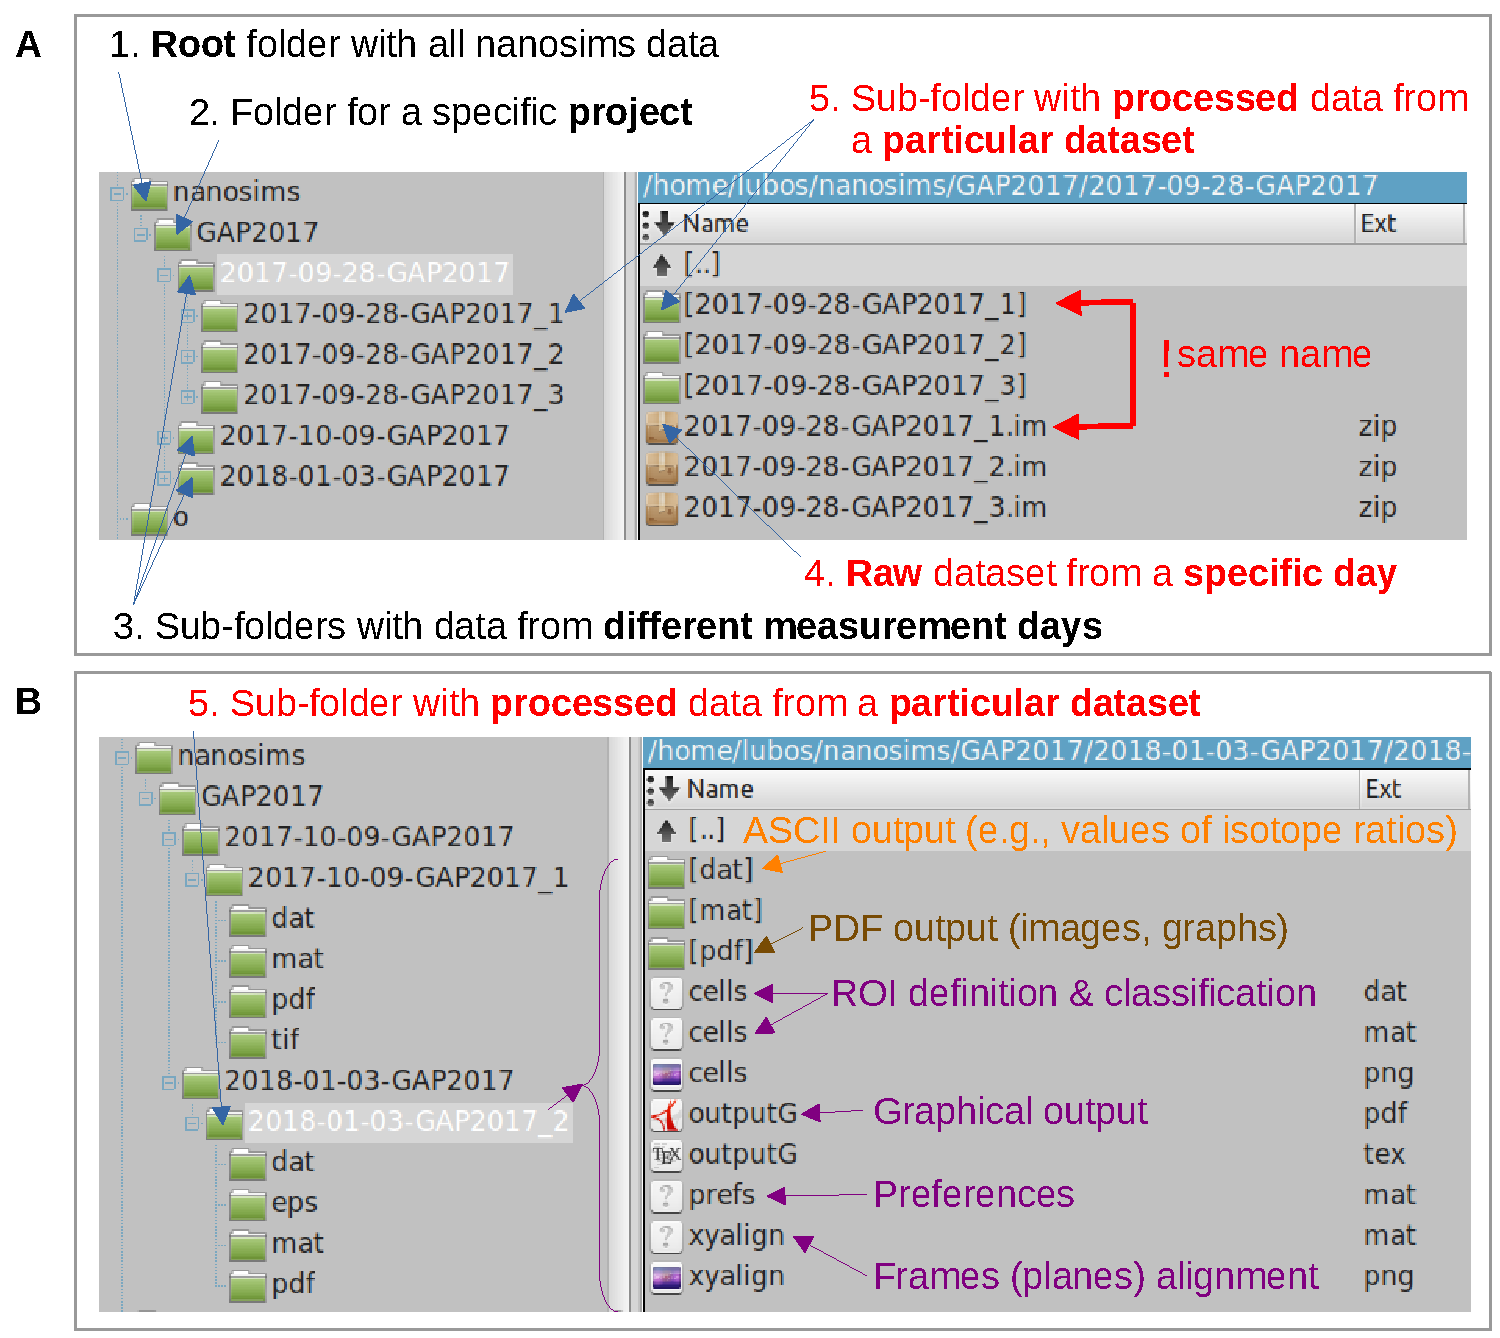
\includegraphics[scale=0.5]{figs2/folders_organizationAB}
\caption{\label{fig2:data_organizationAB}%
	Example of a hierarchical organization of the raw and processed nanoSIMS data implemented in Look@NanoSIMS. %
  \textbf{(A)} The root folder (\ttt{nanosims}) contains a~project-specific sub-folder (e.g., \ttt{GAP2017}), which contains sub-folders with data measured on different days (e.g., \ttt{2017-09-28-GAP2017}, \ttt{2017-10-09-GAP2017}). %
  The `day folder' contains \emph{multiple raw datasets} measured on that particular day (\ttt{im} or \ttt{im.zip} files). %
  When a particular raw dataset is processed and analyzed, the data is stored in a `dataset folder' with the \emph{same name} as the dataset (see red ``!''). %
  \textbf{(B)} The `dataset folder' contains files defining the processing steps, including alignment information (\ttt{xyalign}), definition and classification of regions of interest (\ttt{cells.mat} and \ttt{cells.dat}, respectively), preferences (\ttt{prefs.mat}), and a comprehensive summary of results exported in a PDF file (\ttt{OutputG.pdf}). %
  See more information in Fig.~\ref{fig2:data_organizationCD}.%
}
\end{figure}


\begin{figure}[ht]
\centering
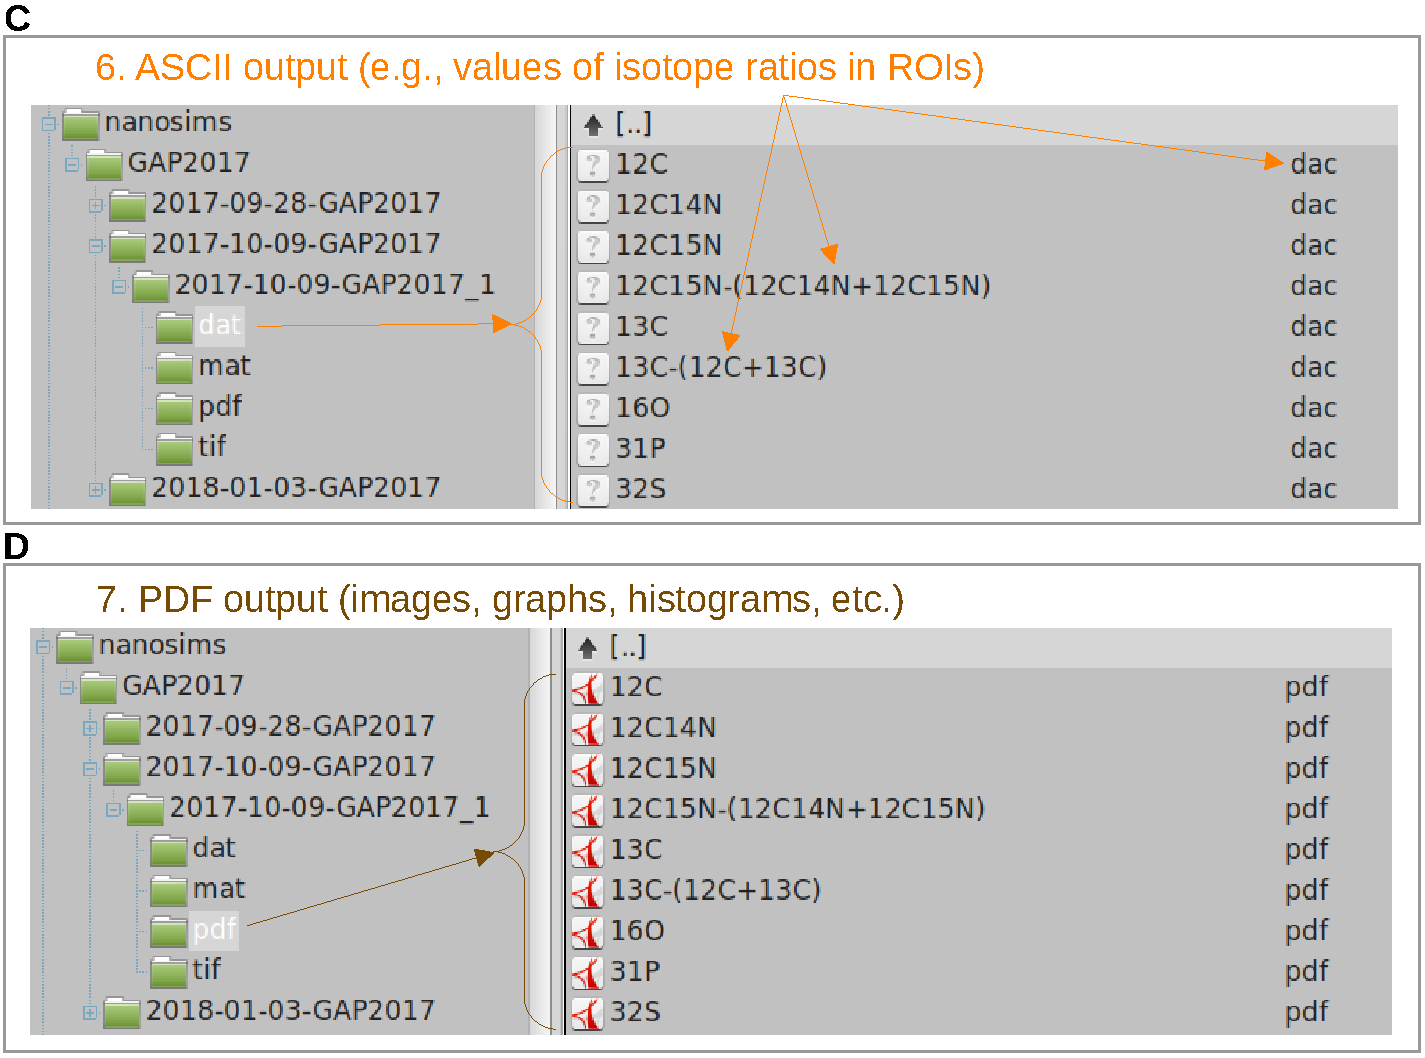
\includegraphics[scale=0.5]{figs2/folders_organizationCD}
\caption{\label{fig2:data_organizationCD}%
  Continuation from Fig.~\ref{fig2:data_organizationAB}. %
The `dataset folder' also contains sub-folders with output generated by LANS in different formats. %
    \textbf{(C)} The ROI-specific ion counts and ion count ratios (\ttt{dac} files) are stored in the \ttt{dat} folder. %
    \textbf{(D)} The images, graphs, histograms, etc., are stored in the \ttt{pdf} folder.}
\end{figure}
